\section{eBPF Setup}\label{sec:ebpf_setup}
TODO

In order to make the congestion control algorithm that is running in userspace
usable we need to inform the QUIC library about the forwarded packets.
This again happens via BPF maps and a separate go routine that continuously
polls new entries in the map and processes them.
Entries are then added to the packet history to allow the receipt of ACKs.
Besides that, the congestion control algorithm will be informed about the
forwarded packet in order to be able to react to potential congestion events.
\begin{figure}[htbp]
    \centering
    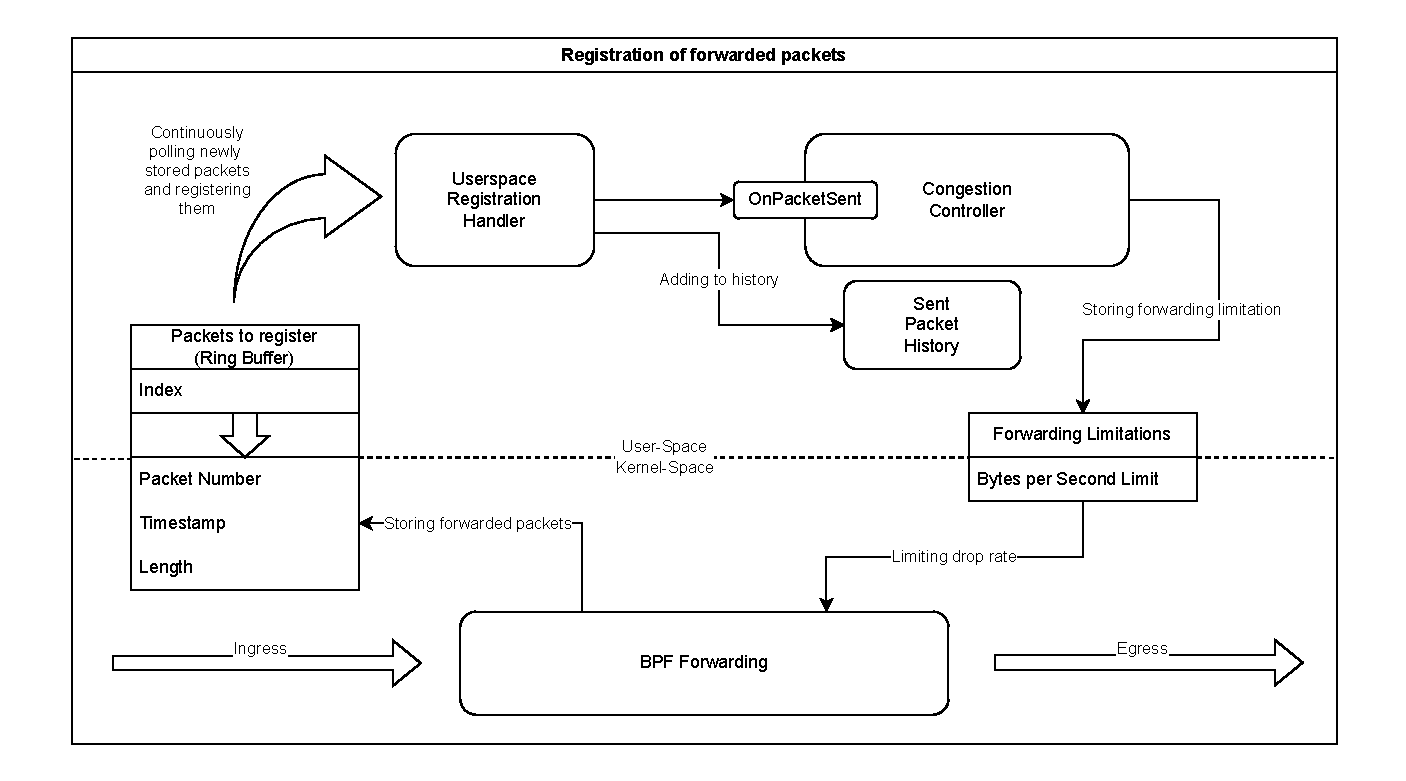
\includegraphics[width=\textwidth]{figures/03_fast_relays/forward-registration.drawio.pdf}
    \caption{Internal setup for registering forwarded packets as well as incorporating forwarding
    limitations for the BPF program.}\label{fig:ebpf-hooks}
\end{figure}